\documentclass[aspectratio=169]{beamer}
\usetheme[theme=blue,logo=logowithtextvi]{HUST} 
\DeclareUnicodeCharacter{221E}{\ensuremath{\infty}}

\usepackage[T5]{fontenc}
\usepackage[utf8]{inputenc}
\usepackage{amsmath}
\usepackage{amsfonts}
\usepackage{amssymb}
\usepackage{graphicx}
\usepackage{adjustbox}
\usepackage{xcolor}
\usepackage{tikz}
\usepackage{minted}
\usepackage{tcolorbox}

\usetikzlibrary{positioning,calc,shapes.symbols, matrix,fit,backgrounds, decorations.pathreplacing}
\definecolor{codeblue}{RGB}{0,90,200}   
\definecolor{codegold}{RGB}{210,160,0}
\definecolor{HUSTBlue}{RGB}{0,51,102}

% ===== Sudoku grid with row/col indices + 3x3 block braces =====






\setminted{
	breaklines=false,
	autogobble=false,
	obeytabs=true,
	tabsize=2,
	linenos=true,
	showspaces=false,
	space=~,
	baselinestretch=1,
	fontsize=\normalsize,
	rulecolor=\color{black}
}

\newcommand{\placecontent}[4]{%
	\tikz[remember picture,overlay]
	\node[anchor=north west]
	at ([xshift=#1,yshift=-#2]current page.north west)
	{\parbox{#3}{#4}};
}

\graphicspath{{./week 5 resources/}}

\title{\huge CẤU TRÚC DỮ LIỆU VÀ GIẢI THUẬT}
\author{SoICT - HUST}
\date{}

\begin{document}
	
	% 2 slides đầu tiên:
	\HUSTInsertBrandSlide
	\HUSTInsertThemeSlide
	
	% Slide tiêu đề
	{\HUSTUseBackground{onelove.pdf}
		\begin{frame}
			\ifdefstring{\insertaspectratio}{169}{
				\HUSTCornerImage[0.14]{assets/logo/soict_vi_h.pdf}
				\placecontent{0.5cm}{0.33\paperheight}{0.85\paperwidth}{
					\color{\HUSTFrameTitleTextColor}\bfseries\fontsize{22pt}{30pt}\selectfont
					\inserttitle
				}
				\placecontent{0.5cm}{0.50\paperheight}{0.8\paperwidth}{
					\color{\HUSTFrameTitleTextColor}\fontsize{14pt}{14pt}\selectfont
					%Bài học
					\textbf{\large TUẦN 5: SƠ ĐỒ THUẬT TOÁN THAM LAM, CHIA ĐỂ TRỊ}\\
				}
			}{}
		\end{frame}
	}
	
	% Outline
	\AtBeginSection[]
	{
		\begin{frame}<beamer>
			\frametitle{NỘI DUNG}
			\tableofcontents[currentsection]
		\end{frame}
	}
	
	%Nội dung chính trong slides
	
	\section{Thuật toán tham lam}
	\begin{frame}[t]{Giới thiệu}
		\setlength{\leftmargini}{-1.2em}
		\small
		
		\begin{itemize}
			\item \textcolor{HUSTBlue}{Thuật toán tham lam} (Greedy algorithm) là cách tiếp cận
			\textcolor{codegold}{đơn giản và có tính trừu tượng cao} để giải
			các bài toán tối ưu, đặc biệt là tối ưu tổ hợp.
			
			\vspace*{0.4cm}
			\item Quá trình tìm lời giải bằng thuật toán tham lam được
			\textcolor{codegold}{chia thành nhiều giai đoạn}
		\end{itemize}
		
		\vspace*{0.35cm}
		
		\centering
		\begin{tikzpicture}[
			decision/.style={
				signal,
				signal from=west,
				signal to=east,
				draw,
				thick,
				fill=white,
				minimum height=1.05cm,
				text height=1.8ex,
				text depth=.25ex,
				font=\bfseries
			}
			]
			\node[decision, minimum width=3.3cm] (d1) {Quyết định 1};
			\node[decision, minimum width=3.3cm, right=-1.8mm of d1] (d2) {Quyết định 2};
			\node[decision, minimum width=2.4cm, right=-1.8mm of d2] (dd) {$\cdots$};
			\node[decision, minimum width=3.3cm, right=-1.8mm of dd] (dn) {Quyết định n};
		\end{tikzpicture}
		
		\vspace*{0.35cm}
		
		% (Đúng như ảnh: lặp lại 2 ý dưới sơ đồ)
		\begin{itemize}
			\item \textcolor{HUSTBlue}{Thuật toán tham lam} (Greedy algorithm) là cách tiếp cận
			\textcolor{codegold}{đơn giản và có tính trừu tượng cao} để giải
			các bài toán tối ưu, đặc biệt là tối ưu tổ hợp.
			
			\vspace*{0.4cm}
			\item Quá trình tìm lời giải bằng thuật toán tham lam được
			\textcolor{codegold}{chia thành nhiều giai đoạn}
		\end{itemize}
	\end{frame}
	
\begin{frame}[t,fragile]{Sơ đồ thuật toán}
	\small
	\setlength{\leftmargini}{-1.2em}
	
	\begin{columns}[T,onlytextwidth]
		
		% ===== CỘT TRÁI =====
		\begin{column}{0.56\textwidth}
			\setlength{\leftmargini}{-1.2em}
			\begin{itemize}
				\item Ký hiệu:
				\begin{itemize}
					\item $S$: Lời giải cần tìm
					\item $C$: Tập các ứng cử viên
					\item \textit{select}$(C)$: Hàm chọn ra ứng cử viên tiềm năng nhất
					\item \textit{solution}$(S)$: TRUE nếu $S$ là lời giải hợp lệ, ngược lại FALSE
					\item \textit{feasible}$(S)$: TRUE nếu $S$ không vi phạm ràng buộc, ngược lại FALSE
				\end{itemize}
			\end{itemize}
		\end{column}
		
		% ===== CỘT PHẢI =====
		\begin{column}{0.44\textwidth}
			\vspace{0.2em}
			\centering
			\begin{minipage}[t]{0.98\textwidth}
				\begin{minted}[
					fontsize=\scriptsize,
					frame=single,
					rulecolor=\color{green!60!black},
					framesep=2mm,
					numbers=none,
					autogobble=true,
					baselinestretch=1.25,
					formatcom=\color{black}\bfseries
					]{text}
					Greedy() {
						S = {};
						while C != {} and not solution(S) {
							x = select(C);
							C = C \ {x};
							if feasible(S U {x}) {
								S = S U {x};
							}
						}
						return S;
					}
				\end{minted}
			\end{minipage}
		\end{column}
		
	\end{columns}
\end{frame}

\begin{frame}[t]{Sơ đồ chung thuật toán}
	\small
	\centering
	
	\begin{tikzpicture}[
		x=1cm,y=1cm,
		scale=0.90,transform shape, % <-- thu nhỏ toàn bộ để khỏi tràn
		box/.style={draw, thick, align=center, minimum width=6.1cm, minimum height=1.0cm},
		>=latex
		]
		% ====== CỘT TRÁI ======
		\node[box, anchor=north west, text=black] (b1) at (0,3.85)
		{Khởi tạo, tập lời giải rỗng};
		
		\node[box, below=0.55cm of b1, text=black] (b2)
		{Chừng nào tập ứng cử viên còn khác rỗng\\
			và {\color{codegold}$S$} chưa phải là lời giải hợp lệ};
		
		\node[box, below=0.55cm of b2, text=black] (b3)
		{Lựa chọn {\color{codegold}$x$} là ứng cử viên tiềm năng nhất\\
			và loại {\color{codegold}$x$} khỏi tập ứng cử viên {\color{codegold}$C$}};
		
		\node[box, below=0.55cm of b3, text=black] (b4)
		{Nếu bổ sung {\color{codegold}$x$} vào lời giải đang xây dựng\\
			nếu không vi phạm ràng buộc};
		
		
		% ====== CỘT PHẢI: CODE (kéo trái + lên một chút) ======
		\matrix (code) [
		matrix of nodes,
		nodes={
			anchor=west,
			font=\ttfamily\scriptsize, % <-- bỏ \bfseries cho đỡ rộng
		},
		row sep=0.03em,              % <-- giảm khoảng dòng
		draw=green!60!black,
		thick,
		inner xsep=6pt,
		inner ysep=5pt,
		anchor=north west
		] at (7.05,3.95) {              % <-- x,y mới (đỡ tràn)
			Greedy() \{ \\
			\ \ \ \ $S=\emptyset$; \\
			\ \ \ \ while $C\neq \emptyset$ and not solution($S$)\{ \\
			\ \ \ \ \ \ \ \ $x$ = select($C$); \\
			\ \ \ \ \ \ \ \ $C = C \setminus \{x\}$; \\
			\ \ \ \ \ \ \ \ if feasible($S \cup \{x\}$) \{ \\
			\ \ \ \ \ \ \ \ \ \ \ \ $S = S \cup \{x\}$; \\
			\ \ \ \ \ \ \ \ \} \\
			\ \ \ \ \} \\
			\ \ \ \ return $S$; \\
			\} \\
		};
		
		% ====== KHUNG ĐỎ (giảm padding + tách rõ, không đè) ======
		\draw[red, thick]
		([xshift=-2pt,yshift=2pt]code-4-1.north west) rectangle
		([xshift= 82pt,yshift=0pt]code-5-1.south east);
		
		% Khung thứ 2 nên bao trọn if + dòng S + dấu } của if (đến dòng 8)
	\draw[red, thick]
	([xshift=-2pt,yshift=-2pt]code-6-1.north west) rectangle
	([xshift= 132pt,yshift=20pt]code-8-1.south east);
	
	% ====== ĐƯỜNG NỐI ======
	\draw[thick] (b1.east) -- ([xshift=-2pt]code-2-1.west);
	\draw[thick] (b2.east) -- ([xshift=-2pt]code-3-1.west);
	
	\coordinate (midSel) at ($(code-4-1.west)!0.5!(code-5-1.west)$);
	\draw[thick] (b3.east) -- ([xshift=-2pt]midSel);
	
	\coordinate (midIf) at ($(code-6-1.west)!0.5!(code-8-1.west)$);
	\draw[thick] (b4.east) -- ([xshift=-2pt]midIf);
	
\end{tikzpicture}
\end{frame}

\begin{frame}[t]{Đặc điểm}
	\small
	\setlength{\leftmargini}{-1.2em}
	
	\begin{columns}[T,onlytextwidth]
		\begin{column}{0.70\textwidth}
			\begin{itemize}
				\item Thuật toán đơn giản $\Rightarrow$ Dễ đề xuất và cài đặt
				\vspace{0.6cm}
				
				\item Trong một số bộ dữ liệu đầu vào và bài toán, thuật toán tham lam cho lời giải tối ưu.
				Tuy nhiên, đa số trường hợp, đặc biệt là các bài toán thực tế có độ phức tạp cao,
				thuật toán này không đảm bảo lời giải trả ra là tối ưu
				\vspace{0.6cm}
				
				\item Thuật toán khá hiệu quả trong những bài toán thực tế có nhiều ràng buộc
				và độ phức tạp cao.
			\end{itemize}
		\end{column}
		
		\begin{column}{0.30\textwidth}
			\centering
			\vspace{1.0cm}
			\includegraphics[width=0.9\linewidth]{greedy_cycle.png}
		\end{column}
	\end{columns}
\end{frame}

\begin{frame}[t]{Ví dụ: Người giao hàng}
	\small
	\setlength{\leftmargini}{-1.2em}
	
	\begin{columns}[T,onlytextwidth]
		% ===== CỘT TRÁI: bullet =====
		\begin{column}{0.62\textwidth}
			\begin{itemize}
				\item Bài toán người bán hàng (Traveling Salesman Problem -- TSP) là
				một bài toán tối ưu kinh điển trong lĩnh vực tối ưu tổ hợp
				
				\vspace{0.35cm}
				\item Bài toán thuộc lớp NP-Hard (Chưa tồn tại thuật toán chạy trong
				thời gian đa thức giải hiệu quả)
				
				\vspace{0.35cm}
				\item Phát biểu: Người bán hàng cần tìm một hành trình qua một tập
				hợp các thành phố sao cho hành trình có tổng chi phí di chuyển là
				nhỏ nhất và mỗi thành phố chỉ được ghé qua đúng một lần trước
				khi quay về thành phố xuất phát.
			\end{itemize}
		\end{column}
		
		% ===== CỘT PHẢI: ảnh + nguồn (click được) =====
		\begin{column}{0.38\textwidth}
			\centering
			\vspace{0.2cm}
			
			% --- bạn tự thay tên file ảnh ---
			\includegraphics[width=\linewidth]{tsp_vn.png}
			
		\end{column}
	\end{columns}
\end{frame}

\begin{frame}[t]{Ví dụ: Người giao hàng}
	\small
	\setlength{\leftmargini}{-1.2em}
	
	\begin{columns}[T,onlytextwidth]
		% ===== CỘT TRÁI =====
		\begin{column}{0.62\textwidth}
			\begin{itemize}
				\item \textbf{Thiết kế:}
				\vspace{0.25cm}
				
				\begin{itemize}
					\setlength{\itemsep}{0.55cm}
					
					\item[\(\blacksquare\)] \textbf{{\color{black}$S$}}: Lời giải cần tìm
					
					\item[\(\blacksquare\)] \textbf{{\color{black}$C$}}: Tập các ứng cử viên
					
					\item[\(\blacksquare\)] \textbf{\textit{select}}\(({\color{black}C})\):
					Hàm chọn ra ứng cử viên tiềm năng nhất
					
					\item[\(\blacksquare\)] \textbf{\textit{solution}}\(({\color{black}S})\):
					Hàm trả về TRUE nếu {\color{codegold}$S$} là một lời giải hợp lệ,
					ngược lại hàm trả về FALSE
					
					\item[\(\blacksquare\)] \textbf{\textit{feasible}}\(({\color{black}S})\):
					Hàm trả về TRUE nếu {\color{codegold}$S$} không vi phạm ràng buộc,
					ngược lại hàm trả về FALSE
				\end{itemize}
			\end{itemize}
		\end{column}
		
		% ===== CỘT PHẢI: VẼ ĐỒ THỊ =====
		\begin{column}{0.38\textwidth}
			\centering
			\vspace{0.2cm}
			
			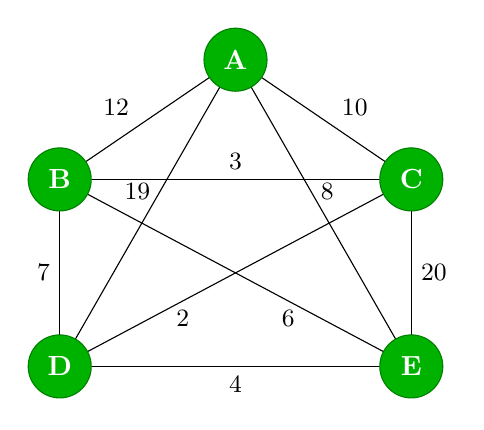
\begin{tikzpicture}[font=\small, line cap=round, line join=round, scale=0.95]
				% ---- tọa độ 5 đỉnh (đặt giống hình) ----
				\coordinate (A) at (0,  2.35);
				\coordinate (B) at (-2.35, 0.75);
				\coordinate (C) at ( 2.35, 0.75);
				\coordinate (D) at (-2.35,-1.75);
				\coordinate (E) at ( 2.35,-1.75);
				
				% ---- vẽ các cạnh (đủ 10 cạnh) + trọng số ----
				\draw (A)--(B) node[pos=0.55, above left] {12};
				\draw (A)--(C) node[pos=0.55, above right]{10};
				
				\draw (B)--(D) node[pos=0.50, left]      {7};
				\draw (C)--(E) node[pos=0.50, right]     {20};
				\draw (D)--(E) node[pos=0.50, below]     {4};
				
				\draw (B)--(C) node[pos=0.50, above]     {3};
				
				\draw (A)--(D) node[pos=0.43, left]      {19};
				\draw (A)--(E) node[pos=0.43, right]     {8};
				
				\draw (C)--(D) node[pos=0.65, below]     {2};
				\draw (B)--(E) node[pos=0.65, below]     {6};
				
				% ---- vẽ các nút (vẽ sau để đè lên cạnh) ----
				\tikzset{city/.style={circle, draw=green!50!black, fill=green!70!black,
						minimum size=8mm, inner sep=0pt, text=white, font=\bfseries}}
				\node[city] at (A) {A};
				\node[city] at (B) {B};
				\node[city] at (C) {C};
				\node[city] at (D) {D};
				\node[city] at (E) {E};
			\end{tikzpicture}
		\end{column}
	\end{columns}
\end{frame}

\begin{frame}[t]{Ví dụ: Người giao hàng}
	\small
	\setlength{\leftmargini}{-1.2em}
	
	\begin{itemize}
		\item[$\blacksquare$] \textbf{Bài toán:} Thiết kế thuật toán tham lam cho bài toán TSP
	\end{itemize}
	
	\begin{columns}[T,onlytextwidth]
		% ================== CỘT TRÁI: 5 HỘP ==================
		\begin{column}{0.42\textwidth}
			\raggedright
			\hspace*{-0.9cm}
			\begin{tikzpicture}[remember picture,
				box/.style={
					draw, thick, align=center,
					text width=6cm,
					text height=0.4cm,
				}
				]
				\node[box] (b1) at (0,0) {Tập con các cạnh của đồ thị};
				\node[box, below=0.22cm of b1] (b2) {Tập tất cả các cạnh của đồ thị};
				\node[box, below=0.22cm of b2] (b3) {Cạnh có trọng số nhỏ nhất};
				
				\node[box, below=0.22cm of b3] (b4)
				{Các cạnh trong \textcolor{orange!85!black}{$S$} tạo thành một chu trình, mỗi đỉnh xuất hiện đúng 1 lần};
				
				\node[box, below=0.22cm of b4] (b5)
				{Các cạnh trong \textcolor{orange!85!black}{$S$} có khả năng tạo thành một chu trình khép kín, chứa mỗi đỉnh đúng một lần};
			\end{tikzpicture}
		\end{column}
		\hspace*{1cm}
		% ================== CỘT PHẢI: THIẾT KẾ ==================
		\begin{column}{0.58\textwidth}
			\begin{itemize}
				\item \textcolor{HUSTBlue}{\textbf{Thiết kế:}}
				
				\vspace{0.20cm}
				
				\item[$\blacksquare$] \tikz[remember picture]\node[coordinate] (tS) {};
				\textbf{{\color{black}$S$}}: \textcolor{HUSTBlue}{Lời giải cần tìm}
				
				\vspace{0.20cm}
				
				\item[$\blacksquare$] \tikz[remember picture]\node[coordinate] (tC) {};
				\textbf{{\color{black}$C$}}: \textcolor{HUSTBlue}{Tập các các ứng cử viên}
				
				\vspace{0.20cm}
				
				\item[$\blacksquare$] \tikz[remember picture]\node[coordinate] (tSel) {};
				\textbf{\textit{select}}$({\color{black}C})$:
				\textcolor{HUSTBlue}{Hàm chọn ra ứng cử viên tiềm năng nhất}
				
				\vspace{0.20cm}
				
				\item[$\blacksquare$] \tikz[remember picture]\node[coordinate] (tSol) {};
				\textbf{\textit{solution}}$({\color{black}S})$:
				\textcolor{HUSTBlue}{Hàm trả về TRUE nếu \textcolor{orange!85!black}{$S$} là một lời giải \\hợp lệ,
					ngược lại hàm trả về FALSE}
				
				\vspace{0.20cm}
				
				\item[$\blacksquare$] \tikz[remember picture]\node[coordinate] (tFea) {};
				\textbf{\textit{feasible}}$({\color{black}S})$:
				\textcolor{HUSTBlue}{Hàm trả về TRUE nếu \textcolor{orange!85!black}{$S$} không vi phạm ràng buộc,
					ngược lại hàm trả về FALSE}
			\end{itemize}
		\end{column}
	\end{columns}
	
	% ================== MŨI TÊN (overlay) ==================
	\begin{tikzpicture}[remember picture, overlay]
		\draw[->, thick] (b1.east) -- ([xshift=-4.1mm,yshift=2mm]tS);
		\draw[->, thick] (b2.east) -- ([xshift=-4.1mm,yshift=2mm]tC);
		\draw[->, thick] (b3.east) -- ([xshift=-4.1mm,yshift=2mm]tSel);
		\draw[->, thick] (b4.east) -- ([xshift=-4.1mm,yshift=2mm]tSol);
		\draw[->, thick] (b5.east) -- ([xshift=-4.1mm,yshift=2mm]tFea);
	\end{tikzpicture}
	
\end{frame}

\begin{frame}[t,fragile]{Ví dụ: Người giao hàng}
	\small
	\setlength{\leftmargini}{-1.2em}
	
	\begin{itemize}
		\item[$\blacksquare$] \textbf{Bài toán:} Thiết kế thuật toán tham lam cho bài toán TSP
		\item \textcolor{HUSTBlue}{\textbf{Biểu diễn thuật toán:}}
	\end{itemize}

	\begin{columns}[T,onlytextwidth]
		% ================== CỘT TRÁI: PSEUDOCODE ==================
		\begin{column}{0.44\textwidth}
			\begin{minted}[
				fontsize=\scriptsize,
				frame=single,
				rulecolor=\color{orange!85!black},
				framesep=2.5mm,
				numbers=none,
				autogobble=true,
				baselinestretch=1.2,
				escapeinside=|| % <-- cho phép chèn LaTeX
				]{text}
				Greedy() {
					S = |\(\emptyset\)|;
					while C |\(\neq\)| |\(\emptyset\)| and not solution(S){
						x = select(C);
						C = C \ {x};
						if feasible(S |\(\cup\)| {x}) {
							S = S |\(\cup\)| {x};
						}
					}
					return S;
				}
			\end{minted}
		\end{column}
		
		% ================== CỘT PHẢI: ĐỒ THỊ + MŨI TÊN VÀNG ==================
		\begin{column}{0.56\textwidth}
			\centering
			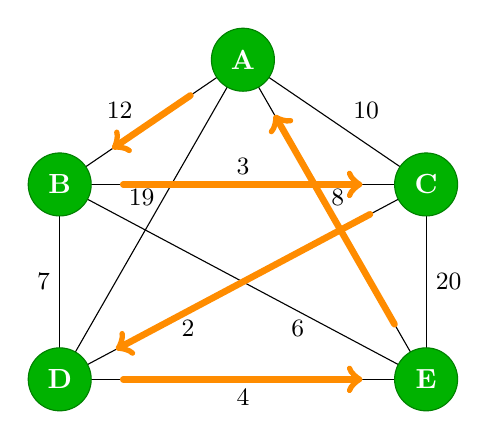
\begin{tikzpicture}[font=\small, line cap=round, line join=round, scale=0.99]
				% ---- tọa độ 5 đỉnh (đặt giống hình) ----
				\coordinate (A) at (0,  2.35);
				\coordinate (B) at (-2.35, 0.75);
				\coordinate (C) at ( 2.35, 0.75);
				\coordinate (D) at (-2.35,-1.75);
				\coordinate (E) at ( 2.35,-1.75);
				
				% ---- vẽ các cạnh (đủ 10 cạnh) + trọng số ----
				\draw (A)--(B) node[pos=0.55, above left] {12};
				\draw (A)--(C) node[pos=0.55, above right]{10};
				
				\draw (B)--(D) node[pos=0.50, left]      {7};
				\draw (C)--(E) node[pos=0.50, right]     {20};
				\draw (D)--(E) node[pos=0.50, below]     {4};
				
				\draw (B)--(C) node[pos=0.50, above]     {3};
				
				\draw (A)--(D) node[pos=0.43, left]      {19};
				\draw (A)--(E) node[pos=0.43, right]     {8};
				
				\draw (C)--(D) node[pos=0.65, below]     {2};
				\draw (B)--(E) node[pos=0.65, below]     {6};
				
				% ---- vẽ các nút (vẽ sau để đè lên cạnh) ----
				\tikzset{city/.style={circle, draw=green!50!black, fill=green!70!black,
						minimum size=8mm, inner sep=0pt, text=white, font=\bfseries}}
				\node[city] (nA) at (A) {A};
				\node[city] (nB) at (B) {B};
				\node[city] (nC) at (C) {C};
				\node[city] (nD) at (D) {D};
				\node[city] (nE) at (E) {E};
				
				% ====== CHỈ BỔ SUNG ĐƯỜNG MŨI TÊN VÀNG (tour) ======
				\draw[->, line width=2.4pt, draw=orange!90!yellow,
				shorten <=4mm, shorten >=4mm]
				(nB) -- (nC);
				
				\draw[->, line width=2.4pt, draw=orange!90!yellow,
				shorten <=4mm, shorten >=4mm]
				(nC) -- (nD);
				
				\draw[->, line width=2.4pt, draw=orange!90!yellow,
				shorten <=4mm, shorten >=4mm]
				(nD) -- (nE);
				
				\draw[->, line width=2.4pt, draw=orange!90!yellow,
				shorten <=4mm, shorten >=4mm]
				(nE) -- (nA);
				
				\draw[->, line width=2.4pt, draw=orange!90!yellow,
				shorten <=4mm, shorten >=4mm]
				(nA) -- (nB);
				
				% (Nếu bạn muốn thêm vòng tròn vàng highlight quanh node như ảnh mẫu, mở comment dưới)
				% \foreach \v in {nA,nB,nC,nD,nE}{
					%   \draw[draw=orange!90!yellow, line width=1.6pt] (\v) circle (6.2mm);
					% }
			\end{tikzpicture}
			
			{\small \textbf{Xuất phát từ:} B$\to$C$\to$D$\to$E$\to$A$\to$B}
		\end{column}
	\end{columns}
\end{frame}

\begin{frame}[t]{Ví dụ: Bài toán tập đoạn con không giao nhau cực đại}
	\small
	\setlength{\leftmargini}{-1.2em}
	
	\begin{itemize}
		\item[$\blacksquare$] \textbf{Bài toán:} Cho tập các đoạn thẳng
		$X=\{(a_1,b_1),\ldots,(a_n,b_n)\}$ trong đó $a_i<b_i,\ \forall i\in\{1,\ldots,n\}$
		là tọa độ hai đầu mút của đoạn thứ $i$ trên đường thẳng.
		Tìm tập con các đoạn đôi một không giao nhau có số lượng phần tử lớn nhất.
	\end{itemize}
	
	\vspace{0.15cm}
	\centering
	
	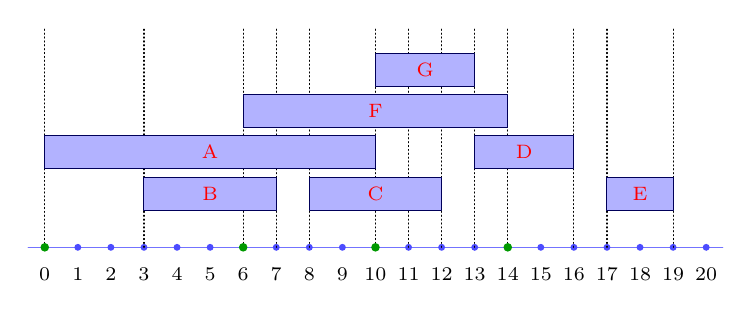
\begin{tikzpicture}[x=0.42cm,y=1.05cm, font=\scriptsize, line cap=round, line join=round]
		% ===== trục số =====
		\draw[blue!55] (-0.5,0) -- (20.5,0);
		
		% chấm xanh dương tại 0..20 + nhãn số
		\foreach \t in {0,1,...,20}{
			\fill[blue!70] (\t,0) circle (1.25pt);
			\node[below=4.0pt] at (\t,0) {\t};
		}
		
		% ===== các vạch dọc chấm (đúng theo hình) =====
		% 0,3,6,7,8,10,11,12,13,14,16,17,19
		\foreach \x in {0,3,6,7,8,10,11,12,13,14,16,17,19}{
			\draw[densely dotted, black] (\x,0) -- (\x,2.65);
		}
		
		% ===== chấm xanh lá (như hình) =====
		\foreach \x in {0,6,10,14}{
			\fill[green!60!black] (\x,0) circle (1.55pt);
		}
		
		% ===== style đoạn =====
		\tikzset{seg/.style={draw=blue!35!black, fill=blue!30, line width=0.35pt}}
		
		% ===== các đoạn (đúng đầu mút) =====
		% (A) [0,10]  -- hàng giữa
		\draw[seg] (0,0.95) rectangle (10,1.35);
		\node[red] at (5,1.15) {A};
		
		% (B) [3,7]   -- hàng thấp
		\draw[seg] (3,0.45) rectangle (7,0.85);
		\node[red] at (5,0.65) {B};
		
		% (C) [8,12]  -- hàng thấp
		\draw[seg] (8,0.45) rectangle (12,0.85);
		\node[red] at (10,0.65) {C};
		
		% (D) [13,16] -- hàng giữa
		\draw[seg] (13,0.95) rectangle (16,1.35);
		\node[red] at (14.5,1.15) {D};
		
		% (E) [17,19] -- hàng thấp (cùng hàng B,C)
		\draw[seg] (17,0.45) rectangle (19,0.85);
		\node[red] at (18,0.65) {E};
		
		% (F) [6,14]  -- hàng cao
		\draw[seg] (6,1.45) rectangle (14,1.85);
		\node[red] at (10,1.65) {F};
		
		% (G) [10,13] -- hàng cao nhất
		\draw[seg] (10,1.95) rectangle (13,2.35);
		\node[red] at (11.5,2.15) {G};
		
	\end{tikzpicture}
	
	\vspace{0.35cm}
	{\large \textcolor{HUSTBlue}{Lời giải tối ưu: $S=\{B,C,D,E\}$}}
	
\end{frame}

\begin{frame}[t]{Ví dụ: Bài toán tập đoạn con không giao nhau cực đại}
	\small
	\setlength{\leftmargini}{-1.2em}
	
	\begin{itemize}
		\item[$\blacksquare$] \textbf{Thiết kế:} Đề xuất thuật toán tham lam 
	\end{itemize}
	
	\begin{columns}[T,onlytextwidth]
		% ================== CỘT TRÁI: 5 HỘP ==================
		\begin{column}{0.42\textwidth}
			\raggedright
			\hspace*{-0.9cm}
				\begin{tikzpicture}[remember picture,
				box/.style={
					draw, thick, align=center,
					text width=6cm,
					text height=0.4cm,
				}
				]
				\node[box] (b1) at (0,0) {Tập con các đoạn thẳng};
				\node[box, below=0.22cm of b1] (b2) {Tập tất cả các đoạn thẳng};
				\node[box, below=0.22cm of b2] (b3) {Đoạn thẳng có ... nhỏ nhất};
				
				\node[box, below=0.22cm of b3] (b4)
				{Đoạn thẳng không giao nhau};
				
				\node[box, below=0.22cm of b4] (b5)
				{Các đoạn thẳng trong \textcolor{red}{$S$} không giao nhau};
			\end{tikzpicture}
		\end{column}
		\hspace*{1cm}
		% ================== CỘT PHẢI: THIẾT KẾ ==================
		\begin{column}{0.58\textwidth}
			\begin{itemize}
				\item \textcolor{HUSTBlue}{\textbf{Thiết kế:}}
				
				\vspace{0.20cm}
				
				\item[$\blacksquare$] \tikz[remember picture]\node[coordinate] (tS) {};
				\textbf{{\color{black}$S$}}: \textcolor{HUSTBlue}{Lời giải cần tìm}
				
				\vspace{0.20cm}
				
				\item[$\blacksquare$] \tikz[remember picture]\node[coordinate] (tC) {};
				\textbf{{\color{black}$C$}}: \textcolor{HUSTBlue}{Tập các các ứng cử viên}
				
				\vspace{0.20cm}
				
				\item[$\blacksquare$] \tikz[remember picture]\node[coordinate] (tSel) {};
				\textbf{\textit{select}}$({\color{black}C})$:
				\textcolor{HUSTBlue}{Hàm chọn ra ứng cử viên tiềm năng nhất}
				
				\vspace{0.20cm}
				
				\item[$\blacksquare$] \tikz[remember picture]\node[coordinate] (tSol) {};
				\textbf{\textit{solution}}$({\color{black}S})$:
				\textcolor{HUSTBlue}{Hàm trả về TRUE nếu \textcolor{orange!85!black}{$S$} là một lời giải \\hợp lệ,
					ngược lại hàm trả về FALSE}
				
				\vspace{0.20cm}
				
				\item[$\blacksquare$] \tikz[remember picture]\node[coordinate] (tFea) {};
				\textbf{\textit{feasible}}$({\color{black}S})$:
				\textcolor{HUSTBlue}{Hàm trả về TRUE nếu \textcolor{orange!85!black}{$S$} không vi phạm ràng buộc,
					ngược lại hàm trả về FALSE}
			\end{itemize}
		\end{column}
	\end{columns}
	
	% ================== MŨI TÊN (overlay) ==================
	\begin{tikzpicture}[remember picture, overlay]
		\draw[->, thick] (b1.east) -- ([xshift=-4.1mm,yshift=2mm]tS);
		\draw[->, thick] (b2.east) -- ([xshift=-4.1mm,yshift=2mm]tC);
		\draw[->, thick] (b3.east) -- ([xshift=-4.1mm,yshift=2mm]tSel);
		\draw[->, thick] (b4.east) -- ([xshift=-4.1mm,yshift=2mm]tSol);
		\draw[->, thick] (b5.east) -- ([xshift=-4.1mm,yshift=2mm]tFea);
	\end{tikzpicture}
	
\end{frame}

\begin{frame}[t]{Ví dụ: Bài toán tập đoạn con không giao nhau cực đại}
	\small
	\centering
	
	\begin{itemize}
		\item[]%
		\hspace*{5cm}% <-- khoảng dịch sang phải của cả khối (bullet + chữ)
		% ô vuông xanh (giống bullet)
		\tikz[baseline=-0.5ex] \fill[HUSTBlue] (0,0) rectangle (0.10,0.10);%
		\hspace{0.6em}%
		% mốc để callout trỏ vào (nằm NGAY SAU bullet, sẽ đi theo dòng)
		\tikz[remember picture,baseline]\node (selAnchor) {};%
		\textbf{\textit{select}$(C)$:}%
		\textcolor{HUSTBlue}{ Hàm chọn ra ứng cử viên tiềm năng nhất}
	\end{itemize}

	

	
	% ===== Callout box bên trái trỏ vào select(C) =====
	\begin{tikzpicture}[remember picture,overlay]
		\node[draw, thick, fill=white, inner xsep=8pt, inner ysep=6pt,
		anchor=west] (callout)
		at ([xshift=1.0cm,yshift=2mm]current page.west |- selAnchor)
		{\textcolor{HUSTBlue}{\textbf{Đoạn thẳng có $a_i$ nhỏ nhất}}};
		
		\draw[thick] (callout.east) -- ([xshift=-3mm,yshift=1.4mm]selAnchor.west);
	\end{tikzpicture}
	
	
	% ===== 2 hình + mũi tên cong =====
	\begin{columns}[T,onlytextwidth]
		% ---- cột trái: mũi tên cong ----
		\begin{column}{0.1\textwidth}
			\centering
			
\begin{tikzpicture}[x=1cm,y=1cm]
				% nền xám dày
				\draw[->, line width=6pt, draw=gray!35]
				(0.9,3.9) .. controls (-0.2,3.2) and (-0.2,2.1) .. (0.9,1.4);
			\end{tikzpicture}
		\end{column}
		
		% ---- cột phải: 2 biểu đồ ----
		\begin{column}{0.9\textwidth}
			\centering
			
			% =================== HÌNH TRÊN (tận dụng code của bạn) ===================
			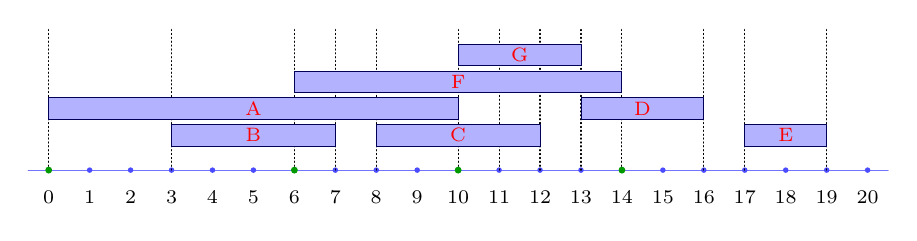
\begin{tikzpicture}[x=0.65cm,y=0.85cm, font=\scriptsize, line cap=round, line join=round, scale=0.8]
				% ===== trục số =====
				\draw[blue!55] (-0.5,0) -- (20.5,0);
				
				% chấm xanh dương tại 0..20 + nhãn số
				\foreach \t in {0,1,...,20}{
					\fill[blue!70] (\t,0) circle (1.25pt);
					\node[below=4.0pt] at (\t,0) {\t};
				}
				
				% ===== các vạch dọc chấm =====
				\foreach \x in {0,3,6,7,8,10,11,12,13,14,16,17,19}{
					\draw[densely dotted, black] (\x,0) -- (\x,2.65);
				}
				
				% ===== chấm xanh lá (như hình trên slide mẫu) =====
				\foreach \x in {0,6,10,14}{
					\fill[green!60!black] (\x,0) circle (1.55pt);
				}
				
				% ===== style đoạn =====
				\tikzset{seg/.style={draw=blue!35!black, fill=blue!30, line width=0.35pt}}
				
				% ===== các đoạn =====
				\draw[seg] (0,0.95) rectangle (10,1.35); \node[red] at (5,1.15) {A};
				\draw[seg] (3,0.45) rectangle (7,0.85);  \node[red] at (5,0.65) {B};
				\draw[seg] (8,0.45) rectangle (12,0.85); \node[red] at (10,0.65) {C};
				\draw[seg] (13,0.95) rectangle (16,1.35);\node[red] at (14.5,1.15) {D};
				\draw[seg] (17,0.45) rectangle (19,0.85); \node[red] at (18,0.65) {E};
				\draw[seg] (6,1.45) rectangle (14,1.85); \node[red] at (10,1.65) {F};
				\draw[seg] (10,1.95) rectangle (13,2.35);\node[red] at (11.5,2.15) {G};
			\end{tikzpicture}
			
	
			
			% =================== HÌNH DƯỚI (kết quả greedy theo a_i nhỏ nhất: A, D, E) ===================
			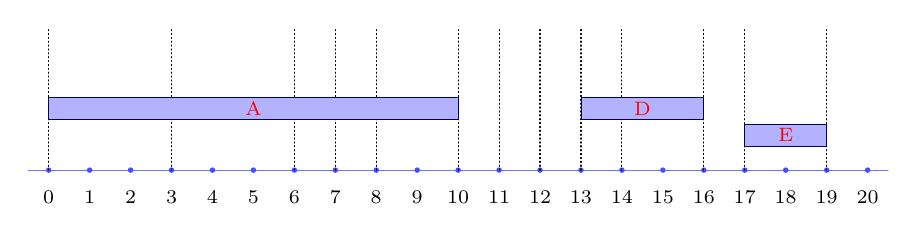
\begin{tikzpicture}[x=0.65cm,y=0.85cm, font=\scriptsize, line cap=round, line join=round, scale=0.8]
				% ===== trục số =====
				\draw[blue!55] (-0.5,0) -- (20.5,0);
				
				% chấm xanh dương tại 0..20 + nhãn số
				\foreach \t in {0,1,...,20}{
					\fill[blue!70] (\t,0) circle (1.25pt);
					\node[below=4.0pt] at (\t,0) {\t};
				}
				
				% ===== các vạch dọc chấm (giữ như hình mẫu) =====
				\foreach \x in {0,3,6,7,8,10,11,12,13,14,16,17,19}{
					\draw[densely dotted, black] (\x,0) -- (\x,2.65);
				}
				
				% ===== style đoạn =====
				\tikzset{seg/.style={draw=blue!35!black, fill=blue!30, line width=0.35pt}}
				
				% ===== chỉ giữ A, D, E =====
				\draw[seg] (0,0.95) rectangle (10,1.35);  \node[red] at (5,1.15) {A};
				\draw[seg] (13,0.95) rectangle (16,1.35); \node[red] at (14.5,1.15) {D};
				\draw[seg] (17,0.45) rectangle (19,0.85); \node[red] at (18,0.65) {E};
			\end{tikzpicture}
			
		\end{column}
	\end{columns}
	
	\begin{itemize}
		\item[] \textcolor{red}{Lời giải này có 3 đoạn $\Rightarrow$ Không tối ưu vì lời giải tối ưu có 4 đoạn ($S=\{B,C,D,E\}$)}
	\end{itemize}

	
\end{frame}

\begin{frame}[t]{Ví dụ: Bài toán tập đoạn con không giao nhau cực đại}
	\small
	\centering
	
	\begin{itemize}
		\item[]%
		\hspace*{5.5cm}% <-- khoảng dịch sang phải của cả khối (bullet + chữ)
		% ô vuông xanh (giống bullet)
		\tikz[baseline=-0.5ex] \fill[HUSTBlue] (0,0) rectangle (0.10,0.10);%
		% mốc để callout trỏ vào (nằm NGAY SAU bullet, sẽ đi theo dòng)
		\tikz[remember picture,baseline]\node (selAnchor) {};%
		\textbf{\textit{select}$(C)$:}%
		\textcolor{HUSTBlue}{ Hàm chọn ứng cử viên tiềm năng nhất}
	\end{itemize}
	
	
	
	
	% ===== Callout box bên trái trỏ vào select(C) =====
	\begin{tikzpicture}[remember picture,overlay]
		\node[draw, thick, fill=white, inner xsep=8pt, inner ysep=6pt,
		anchor=west] (callout)
		at ([xshift=1.0cm,yshift=2mm]current page.west |- selAnchor)
		{\textcolor{HUSTBlue}{\textbf{Đoạn thẳng có $b_i$ - $a_i$ nhỏ nhất}}};
		
		\draw[thick] (callout.east) -- ([xshift=-3mm,yshift=1.4mm]selAnchor.west);
	\end{tikzpicture}
	
	
	% ===== 2 hình + mũi tên cong =====
	\begin{columns}[T,onlytextwidth]
		% ---- cột trái: mũi tên cong ----
		\begin{column}{0.1\textwidth}
			\centering
			
\begin{tikzpicture}[x=1cm,y=1cm]
				% nền xám dày
				\draw[->, line width=6pt, draw=gray!35]
				(0.9,3.9) .. controls (-0.2,3.2) and (-0.2,2.1) .. (0.9,1.4);
			\end{tikzpicture}
		\end{column}
		
		% ---- cột phải: 2 biểu đồ ----
		\begin{column}{0.9\textwidth}
			\centering
			
			% =================== HÌNH TRÊN (tận dụng code của bạn) ===================
			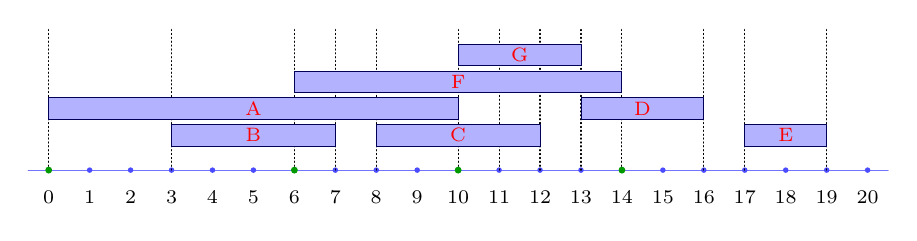
\begin{tikzpicture}[x=0.65cm,y=0.85cm, font=\scriptsize, line cap=round, line join=round, scale=0.8]
				% ===== trục số =====
				\draw[blue!55] (-0.5,0) -- (20.5,0);
				
				% chấm xanh dương tại 0..20 + nhãn số
				\foreach \t in {0,1,...,20}{
					\fill[blue!70] (\t,0) circle (1.25pt);
					\node[below=4.0pt] at (\t,0) {\t};
				}
				
				% ===== các vạch dọc chấm =====
				\foreach \x in {0,3,6,7,8,10,11,12,13,14,16,17,19}{
					\draw[densely dotted, black] (\x,0) -- (\x,2.65);
				}
				
				% ===== chấm xanh lá (như hình trên slide mẫu) =====
				\foreach \x in {0,6,10,14}{
					\fill[green!60!black] (\x,0) circle (1.55pt);
				}
				
				% ===== style đoạn =====
				\tikzset{seg/.style={draw=blue!35!black, fill=blue!30, line width=0.35pt}}
				
				% ===== các đoạn =====
				\draw[seg] (0,0.95) rectangle (10,1.35); \node[red] at (5,1.15) {A};
				\draw[seg] (3,0.45) rectangle (7,0.85);  \node[red] at (5,0.65) {B};
				\draw[seg] (8,0.45) rectangle (12,0.85); \node[red] at (10,0.65) {C};
				\draw[seg] (13,0.95) rectangle (16,1.35);\node[red] at (14.5,1.15) {D};
				\draw[seg] (17,0.45) rectangle (19,0.85); \node[red] at (18,0.65) {E};
				\draw[seg] (6,1.45) rectangle (14,1.85); \node[red] at (10,1.65) {F};
				\draw[seg] (10,1.95) rectangle (13,2.35);\node[red] at (11.5,2.15) {G};
			\end{tikzpicture}
			
			
			
			% =================== HÌNH DƯỚI (kết quả greedy theo a_i nhỏ nhất: A, D, E) ===================
			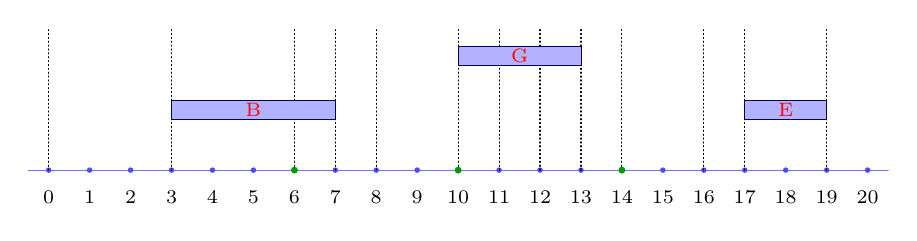
\begin{tikzpicture}[x=0.65cm,y=0.85cm, font=\scriptsize, line cap=round, line join=round, scale=0.8]
				% ===== trục số =====
				\draw[blue!55] (-0.5,0) -- (20.5,0);
				
				% ===== chấm xanh dương + nhãn dưới (0..20) =====
				\foreach \t in {0,1,...,20}{
					\fill[blue!70] (\t,0) circle (1.25pt);
					\node[below=4.0pt] at (\t,0) {\t};
				}
				
				
				% ===== các vạch dọc chấm (như bộ của bạn) =====
				\foreach \x in {0,3,6,7,8,10,11,12,13,14,16,17,19}{
					\draw[densely dotted, black] (\x,0) -- (\x,2.65);
				}
				
				% ===== chấm xanh lá (như hình) =====
				\foreach \x in {6,10,14}{
					\fill[green!60!black] (\x,0) circle (1.55pt);
				}
				
				% ===== style đoạn =====
				\tikzset{seg/.style={draw=blue!35!black, fill=blue!30, line width=0.35pt}}
				
				% ===== các đoạn cần vẽ: B, G, E =====
				% B: [3,7] (hàng thấp)
				\draw[seg] (3,0.95) rectangle (7,1.30);
				\node[red] at (5,1.125) {B};
				
				% G: [10,13] (hàng cao)
				\draw[seg] (10,1.95) rectangle (13,2.30);
				\node[red] at (11.5,2.125) {G};
				
				% E: [17,19] (hàng thấp)
				\draw[seg] (17,0.95) rectangle (19,1.30);
				\node[red] at (18,1.125) {E};
			\end{tikzpicture}
			
		\end{column}
	\end{columns}
	
	\begin{itemize}
		\item[] \textcolor{red}{Lời giải này có 3 đoạn $\Rightarrow$ Không tối ưu vì lời giải tối ưu có 4 đoạn ($S=\{B,C,D,E\}$)}
	\end{itemize}
	
	
\end{frame}


\begin{frame}[t]{Ví dụ: Bài toán tập đoạn con không giao nhau cực đại}
	\small
	\centering
	
	\begin{itemize}
		\item[]%
		\hspace*{5.5cm}% <-- khoảng dịch sang phải của cả khối (bullet + chữ)
		% ô vuông xanh (giống bullet)
		\tikz[baseline=-0.5ex] \fill[HUSTBlue] (0,0) rectangle (0.10,0.10);%
		% mốc để callout trỏ vào (nằm NGAY SAU bullet, sẽ đi theo dòng)
		\tikz[remember picture,baseline]\node (selAnchor) {};%
		\textbf{\textit{select}$(C)$:}%
		\textcolor{HUSTBlue}{ Hàm chọn ứng cử viên tiềm năng nhất}
	\end{itemize}
	
	
	
	
	% ===== Callout box bên trái trỏ vào select(C) =====
	\begin{tikzpicture}[remember picture,overlay]
		\node[draw, thick, fill=white, inner xsep=8pt, inner ysep=6pt,
		anchor=west] (callout)
		at ([xshift=1.0cm,yshift=2mm]current page.west |- selAnchor)
		{\textcolor{HUSTBlue}{\textbf{Đoạn thẳng có $b_i$ nhỏ nhất}}};
		
		\draw[thick] (callout.east) -- ([xshift=-3mm,yshift=1.4mm]selAnchor.west);
	\end{tikzpicture}
	\vspace{-5mm}
	
	
	% ===== 2 hình + mũi tên cong =====
	\begin{columns}[T,onlytextwidth]
		% ---- cột trái: mũi tên cong ----
		\begin{column}{0.1\textwidth}
			\centering
			
\begin{tikzpicture}[x=1cm,y=1cm]
				% nền xám dày
				\draw[->, line width=6pt, draw=gray!35]
				(0.9,3.9) .. controls (-0.2,3.2) and (-0.2,2.1) .. (0.9,1.4);
			\end{tikzpicture}
		\end{column}
		
		% ---- cột phải: 2 biểu đồ ----
		\begin{column}{0.9\textwidth}
			\centering
			
			% =================== HÌNH TRÊN (tận dụng code của bạn) ===================
			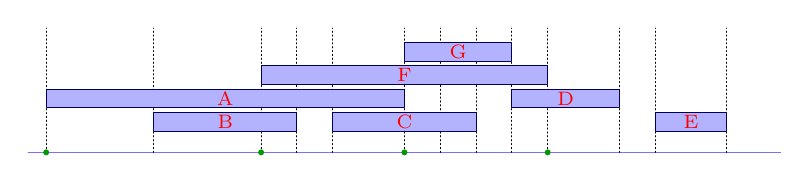
\begin{tikzpicture}[x=0.65cm,y=0.85cm, font=\scriptsize, line cap=round, line join=round, scale=0.7]
				% ===== trục số =====
				\draw[blue!55] (-0.5,0) -- (20.5,0);
	
				
				% ===== các vạch dọc chấm =====
				\foreach \x in {0,3,6,7,8,10,11,12,13,14,16,17,19}{
					\draw[densely dotted, black] (\x,0) -- (\x,2.65);
				}
				
				% ===== chấm xanh lá (như hình trên slide mẫu) =====
				\foreach \x in {0,6,10,14}{
					\fill[green!60!black] (\x,0) circle (1.55pt);
				}
				
				% ===== style đoạn =====
				\tikzset{seg/.style={draw=blue!35!black, fill=blue!30, line width=0.35pt}}
				
				% ===== các đoạn =====
				\draw[seg] (0,0.95) rectangle (10,1.35); \node[red] at (5,1.15) {A};
				\draw[seg] (3,0.45) rectangle (7,0.85);  \node[red] at (5,0.65) {B};
				\draw[seg] (8,0.45) rectangle (12,0.85); \node[red] at (10,0.65) {C};
				\draw[seg] (13,0.95) rectangle (16,1.35);\node[red] at (14.5,1.15) {D};
				\draw[seg] (17,0.45) rectangle (19,0.85); \node[red] at (18,0.65) {E};
				\draw[seg] (6,1.45) rectangle (14,1.85); \node[red] at (10,1.65) {F};
				\draw[seg] (10,1.95) rectangle (13,2.35);\node[red] at (11.5,2.15) {G};
			\end{tikzpicture}
			
			
			
			% =================== HÌNH DƯỚI (kết quả greedy theo a_i nhỏ nhất: A, D, E) ===================
			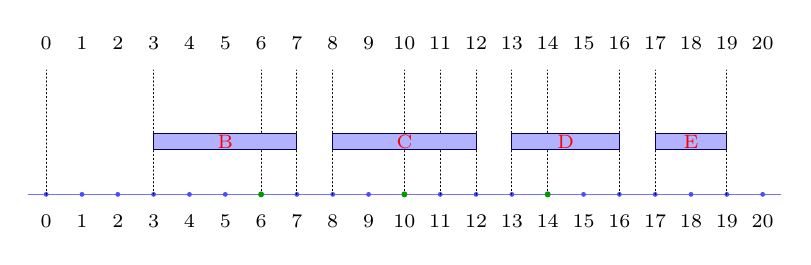
\begin{tikzpicture}[x=0.65cm,y=0.85cm, font=\scriptsize, line cap=round, line join=round, scale=0.7]
				  \draw[blue!55] (-0.5,0) -- (20.5,0);
				
				% ===== chấm xanh dương + nhãn dưới (0..20) =====
				\foreach \t in {0,1,...,20}{
					\fill[blue!70] (\t,0) circle (1.25pt);
					\node[below=4.0pt] at (\t,0) {\t};
				}
				
				% ===== nhãn trên (0..20) =====
				\foreach \t in {0,1,...,20}{
					\node[above=4.0pt] at (\t,2.65) {\t};
				}
				
				% ===== các vạch dọc chấm =====
				\foreach \x in {0,3,6,7,8,10,11,12,13,14,16,17,19}{
					\draw[densely dotted, black] (\x,0) -- (\x,2.65);
				}
				
				% ===== chấm xanh lá =====
				\foreach \x in {6,10,14}{
					\fill[green!60!black] (\x,0) circle (1.55pt);
				}
				
				% ===== style đoạn =====
				\tikzset{seg/.style={draw=blue!35!black, fill=blue!30, line width=0.35pt}}
				
				% ===== các đoạn: B, C, D, E (cùng 1 hàng) =====
				% B: [3,7]
				\draw[seg] (3,0.95) rectangle (7,1.30);
				\node[red] at (5,1.125) {B};
				
				% C: [8,12]
				\draw[seg] (8,0.95) rectangle (12,1.30);
				\node[red] at (10,1.125) {C};
				
				% D: [13,16]
				\draw[seg] (13,0.95) rectangle (16,1.30);
				\node[red] at (14.5,1.125) {D};
				
				% E: [17,19]
				\draw[seg] (17,0.95) rectangle (19,1.30);
				\node[red] at (18,1.125) {E};
			\end{tikzpicture}
			
		\end{column}
	\end{columns}
	
	\begin{itemize}
		\item[] \textcolor{HUSTBlue}{Thuật toán tìm được lời giải tối ưu có 4 đoạn}
		\item[] \textcolor{red}{Btvn: chưng minh thuật toán tham làm này luôn trả ra lời giải tối ưu}
	\end{itemize}
\end{frame}

\begin{frame}[t]{Bài tập luyện tập}
	\small
	\setlength{\leftmargini}{-1.2em}
	
	\begin{itemize}
		\item \textbf{Đề bài:}
		Có $n$ công việc $1,2,\ldots,n$. Công việc $i$ có thời hạn hoàn thành là $d[i]$
		và có lợi nhuận khi được đưa vào thực hiện là $p[i]$ $(i=1,\ldots,n)$.
		Biết rằng chỉ được nhiều nhất $1$ công việc được thực hiện tại mỗi thời điểm
		và thời gian thực hiện xong mỗi công việc đều là $1$ đơn vị.
		Hãy tìm cách chọn ra các công việc để đưa vào thực hiện sao cho tổng lợi nhuận thu được
		là nhiều nhất, đồng thời mỗi công việc phải hoàn thành trước hoặc đúng thời hạn.
		
		\item \textbf{Hình thức:} Làm tại nhà và nộp lại trên hệ thống chấm code.
	\end{itemize}
	
\end{frame}

\section{Thuật toán chia để trị}

\begin{frame}[t]{Giới thiệu}
	\setlength{\leftmargini}{-1.2em}
	\small
	\begin{columns}[T,onlytextwidth]
		% ===== CỘT TRÁI =====
		\begin{column}{0.40\textwidth}
			\begin{itemize}
				\item \textcolor{HUSTBlue}{Thuật toán chia để trị (Divide and Conquer algorithm)} là
				kỹ thuật mạnh trong Khoa học máy tính và Toán học.
				
				\item \textbf{Ý tưởng:} là làm dễ bài toán bằng cách chia nhỏ bài toán
				phức tạp thành những bài toán con đơn giản hơn (CHIA),
				giải riêng rẽ các bài toán con (TRỊ) và cuối cùng là tổng hợp các kết quả
				bài toán con để thu được lời giải bài toán ban đầu.
				\item 	{\footnotesize\textit{Nguồn: }\href{https://www.javatpoint.com/divide-and-conquer-introduction}{https://www.javatpoint.com/divide-and-conquer-introduction}}
			\end{itemize}
		\end{column}
		
		% ===== CỘT PHẢI =====
		\hspace*{0.5cm}
		\begin{column}{0.60\textwidth}
			\centering
			
			% ====== HÌNH Divide & Conquer ======
			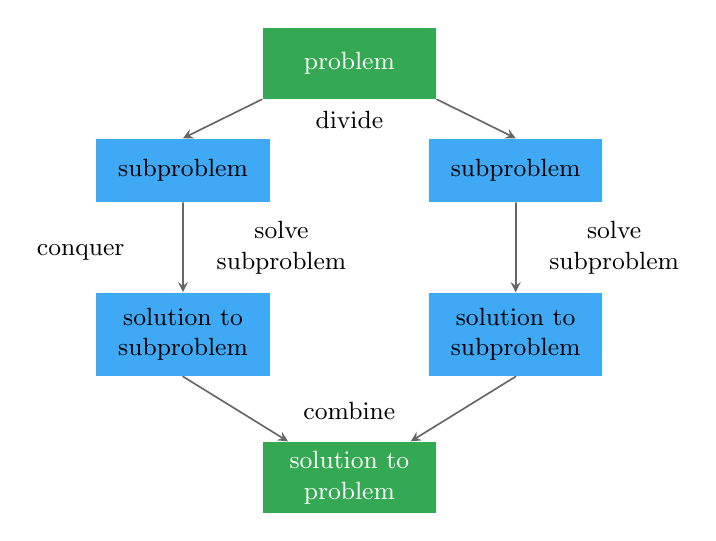
\begin{tikzpicture}[
				font=\small,
				>=stealth,
				line cap=round,
				line join=round,
				scale=0.65,
				every path/.style={draw=black!60, line width=0.6pt}
				]
				% Màu gần giống hình
				\definecolor{dcGreen}{HTML}{34A853}
				\definecolor{dcBlue}{HTML}{3FA9F5}
				
				% Style node
				\tikzset{
					gbox/.style={rectangle, fill=dcGreen, text=white, align=center,
						minimum width=2.2cm, minimum height=0.9cm},
					bbox/.style={rectangle, fill=dcBlue, text=black, align=center,
						minimum width=2.2cm, minimum height=0.8cm},
					bbig/.style={rectangle, fill=dcBlue, text=black, align=center,
						minimum width=2.2cm, minimum height=1.05cm}
				}
				
				% ===== Node positions (đặt giống ảnh) =====
				\node[gbox] (P)  at (0, 3.10) {problem};
				
				\node[bbox] (L1) at (-3.25, 1) {subproblem};
				\node[bbox] (R1) at ( 3.25, 1) {subproblem};
				
				\node[bbig] (L2) at (-3.25, -2.2) {solution to\\subproblem};
				\node[bbig] (R2) at ( 3.25, -2.2) {solution to\\subproblem};
				
				\node[gbox] (S)  at (0, -5.0) {solution to\\problem};
				
				% ===== Arrows + labels =====
				% divide
				\draw[->] (P.south west) -- (L1.north);
				\draw[->] (P.south east) -- (R1.north);
				\node at (0, 2.0) {divide};
				
				% conquer + solve subproblem
				\draw[->] (L1.south) -- (L2.north)
				node[midway, right=3mm, align=center] {solve\\subproblem};
				\draw[->] (R1.south) -- (R2.north)
				node[midway, right=3mm, align=center] {solve\\subproblem};
				
				\node at (-5.25, -0.6) {conquer};
				
				% combine
				\draw[->] (L2.south) -- ([xshift=-12mm]S.north);
				\draw[->] (R2.south) -- ([xshift= 12mm]S.north);
				\node at (0, -3.7) {combine};
				
			\end{tikzpicture}
		\end{column}
	\end{columns}
\end{frame}

\begin{frame}[t,fragile]{Sơ đồ thuật toán}
	\small
	\setlength{\leftmargini}{-1.2em}
	
	\begin{columns}[T,onlytextwidth]
		
		% ===== CỘT TRÁI =====
		\begin{column}{0.46\textwidth}
			\setlength{\leftmargini}{-1.2em}
			\setlength{\itemsep}{0.9em}
			\begin{itemize}
				\item \textbf{Sử dụng thuật toán:} Sử dụng \textcolor{red}{Đệ quy} để thể hiện\\
				sơ đồ chung của thuật toán \textcolor{red}{chia để trị}
				
				\item[$\Rightarrow$] Dễ hiểu và thể hiện rõ ý tưởng của thuật toán
			\end{itemize}
		\end{column}
		\hspace*{0.5cm}
		
		% ===== CỘT PHẢI =====
		\begin{column}{0.54\textwidth}
			\vspace{0.2em}
			\centering
			\begin{minipage}[t]{0.98\textwidth}
			\begin{minted}[
				fontsize=\scriptsize,
				frame=single,
				rulecolor=\color{black!55},
				framesep=2mm,
				numbers=none,
				autogobble=true,
				baselinestretch=1.25,
				escapeinside=||
				]{text}
				|\textbf{\textit{DC}}|(|$P_n$|) {
					|\textit{if}| |$n \le n_0$| {
						|\textit{solve\_problem}|(|$p_n$|);
					} |\textit{else}| {
						|$SP$| = |\textit{divide}|(|$P_n$|);
						|\textit{foreach}| |$p \in SP$| {
							|$s(p)$| = |\textbf{\textit{DC}}|(|$p$|)
						}
						|$S$| = |\textit{aggregate}|(|$s(p_1), \ldots, s(p_k)$|)
					}
					|\textbf{return}| |$S$|;
				}
			\end{minted}
			\end{minipage}
		\end{column}
		
	\end{columns}
\end{frame}

\begin{frame}[t]{Sơ đồ thuật toán}
	\small
	\centering
	
	\begin{tikzpicture}[x=1cm,y=1cm,scale=0.92,transform shape,>=latex]
		
		\tikzset{
			codebox/.style={draw=black, thick, inner xsep=10pt, inner ysep=8pt},
			call/.style={draw=black, thick, fill=white, align=left,
				text width=6.9cm, inner xsep=10pt, inner ysep=8pt}
		}
		
		% ===== KHỐI CODE (TRÁI) =====
		% ===== KHỐI CODE (TRÁI) - bản siết dòng (chỉ ảnh hưởng matrix này) =====
		\matrix (code) [
		matrix of nodes,
		draw=black, thick,
		inner xsep=10pt, inner ysep=6pt,     % padding của KHUNG (giữ vừa phải)
		row sep=1em,                      % <<< siết khoảng giữa các dòng
		column sep=0pt,
		nodes={
			anchor=west,
			font=\ttfamily\scriptsize\linespread{0.82}\selectfont, % <<< siết line spacing
			inner sep=0pt,                                          % <<< bỏ padding từng dòng
			text height=1.15ex, text depth=0.15ex                   % <<< ép chiều cao mỗi dòng
		},
		anchor=north west
		] at (0,6.55) {
			\textbf{\textit{DC}}($P_n$) \{ \\
			\hspace*{1.8em}\textit{if} $n \le n_0$ \{ \\
			\hspace*{3.6em}\textit{solve\_problem}($p_n$); \\
			\hspace*{1.8em}\} \textit{else} \{ \\
			\hspace*{3.6em}$SP$ = \textit{divide}($P_n$); \\
			\hspace*{3.6em}\textit{foreach} $p \in SP$ \{ \\
			\hspace*{5.4em}$s(p)$ = \textbf{\textit{DC}}($p$) \\
			\hspace*{3.6em}\} \\
			\hspace*{3.6em}$S$ = \textit{aggregate}($s(p_1),\ldots,s(p_k)$) \\
			\hspace*{1.8em}\} \\
			\hspace*{1.8em}\textbf{return} $S$; \\
			\} \\
		};
		
		% ===== 4 KHUNG ĐỎ (đúng các đoạn trong ảnh) =====
		\draw[red, thick]
		([xshift=1pt,yshift=5pt]code.west |- code-2-1.north)
		rectangle
		([xshift=-1pt,yshift=-3pt]code.east |- code-3-1.south);
		
		\draw[red, thick]
		([xshift=1pt,yshift=5pt]code.west |- code-6-1.north)
		rectangle
		([xshift=-1pt,yshift=-20pt]code.east |- code-7-1.south);
		
		% ===== 4 HỘP GIẢI THÍCH (PHẢI) - bản siết khoảng trắng =====
		\node[call, minimum height=1.70cm, anchor=north west] (c1)
		at ([xshift=1.45cm,yshift=0.05cm]code.north east)
		{%
			$n_0$ là kích thước nhỏ của bài toán, mà chúng ta\\
			có thể chỉ ra lời giải của bài một cách dễ dàng.\\
			Đây là bước cơ sở trong kỹ thuật Đệ quy.
		};
		
		\node[call, minimum height=0.85cm, anchor=north west] (c2)
		at ([yshift=-0.25cm]c1.south west)
		{Chia nhỏ bài toán cha thành nhiều bài toán con};
		
		\node[call, minimum height=0.85cm, anchor=north west] (c3)
		at ([yshift=-0.25cm]c2.south west)
		{Giải từng bài toán con};
		
		\node[call, minimum height=1.10cm, anchor=north west] (c4)
		at ([yshift=-0.25cm]c3.south west)
		{%
			Tổng hợp kết quả các bài toán con để xây dựng\\
			lời giải bài toán cha (bài toán ban đầu)
		};
		
		% ===== 4 MŨI TÊN TRỎ VỀ CODE (mũi tên hướng sang trái như ảnh) =====
		\coordinate (h1) at ($(code-2-1.east)!0.5!(code-3-1.east)$);
		\coordinate (p1) at (code.east |- h1);
		\draw[->, thick] (c1.west) -- (p1);
		
		\coordinate (h2) at (code-5-1.east);
		\coordinate (p2) at (code.east |- h2);
		\draw[->, thick] (c2.west) -- (p2);
		
		\coordinate (h3) at ($(code-6-1.east)!0.5!(code-7-1.east)$);
		\coordinate (p3) at (code.east |- h3);
		\draw[->, thick] (c3.west) -- (p3);
		
		\coordinate (h4) at (code-9-1.east);
		\coordinate (p4) at (code.east |- h4);
		\draw[->, thick] (c4.west) -- (p4);
		
	\end{tikzpicture}
\end{frame}

\begin{frame}[t]{Đặc điểm}
	\small
	\setlength{\leftmargini}{-1.2em}
	
	\begin{columns}[T,onlytextwidth]
		% ===== CỘT TRÁI: BULLETS =====
		\begin{column}{0.68\textwidth}
			\begin{itemize}
				\item Ý tưởng thuật toán ``Chia nhỏ'' rất tự nhiên và giống với cách tiếp
				cận giải quyết vấn đề của con người
				
				\vspace{0.35cm}
				
				\item Các bài toán con độc lập, có nghĩa là việc giải một bài toán con
				không ảnh hưởng đến giải pháp của các bài toán con đồng mức khác
				
				\vspace{0.35cm}
				
				\item Việc chia bài toán đảm bảo không mất nghiệm
				
				\vspace{0.35cm}
				
				\item Một số ứng dụng nổi bật
				\begin{itemize}
					\item Tính toán song song
					\item Tìm kiếm
				\end{itemize}
			\end{itemize}
		\end{column}
		
		% ===== CỘT PHẢI: ẢNH (bạn tự thay file) =====
		\begin{column}{0.32\textwidth}
			\centering
			\vspace{0.4cm}
			\includegraphics[width=0.95\linewidth]{divide_conquer_icon.png}
		\end{column}
	\end{columns}
	
\end{frame}

\begin{frame}[t]{Ví dụ: Đoạn con có tổng lớn nhất}
	\small
	\setlength{\leftmargini}{-1.2em}
	
	\begin{itemize}
		\item \textbf{Phát biểu:} Cho dãy $n$ số nguyên $(a_1,a_2,\ldots,a_n)$, hãy tìm đoạn con bao gồm các phần tử liên tiếp của
		dãy sao cho tổng các phần tử được chọn là cực đại.
		\vspace*{0.35em}
		
		\item \textbf{Ví dụ:} Cho dãy 7 số nguyên sau
	\end{itemize}
	
	\centering
	
	\begin{tikzpicture}[
		cell/.style={draw, minimum width=1.55cm, minimum height=1.1cm, align=center},
		num/.style={font=\bfseries\Large, text=HUSTBlue},
		brace/.style={decorate, decoration={brace, amplitude=7pt, mirror}, very thick},
		scale=0.95, transform shape
		]
		% ===== 7 ô số (KHÔNG dùng matrix, KHÔNG dùng &) =====
		\foreach \v [count=\i from 1] in {-16,7,-3,0,-1,5,-4}{
			\node[cell] (A\i) at ({(\i-1)*1.55},0) {\textcolor{HUSTBlue}{\bfseries\Large \v}};
		}
		
		% ===== ngoặc đen: -16..0 =====
		\draw[brace, black]
		($(A1.south west)+(0,-0.10)$) -- ($(A4.south east)+(0,-0.10)$);
		\node[font=\bfseries\itshape, black]
		at ($(A1.south west)!0.5!(A4.south east)+(0,-0.95)$)
		{Đoạn con có tổng -12};
		
		% ===== ngoặc đỏ: -1..-4 =====
		\draw[brace, red]
		($(A5.south west)+(0,-0.10)$) -- ($(A7.south east)+(0,-0.10)$);
		\node[font=\bfseries\itshape, red]
		at ($(A5.south west)!0.5!(A7.south east)+(0,-0.95)$)
		{Đoạn con có tổng 0};
		
	\end{tikzpicture}
	
	\begin{itemize}
		\item Lời giải tối ưu (dãy con có tổng cực đại bằng 8): $7,-3,0,-1,5$
		\vspace*{0.35em}
		\item Thuật toán vét cạn có độ phức tạp $O(n^2)$, chúng ta có thể làm tốt hơn với thuật toán chia để trị hay không?
	\end{itemize}
	
\end{frame}

\begin{frame}[t]{Ví dụ: Đoạn con có tổng lớn nhất}
	\small
	\setlength{\leftmargini}{-1.2em}
	
	\begin{itemize}
		\item \textbf{Xác định bài toán con:} Bài toán con của bài toán tìm đoạn con cực đại của dãy
		$(a_1,\ldots,a_n)$ là bài toán tìm đoạn con cực đại của đoạn con
		$a_i,a_{i+1},\ldots,a_{i+j}, i \ge 1,\, i+j \le n$.
	\end{itemize}
	
	\vspace{0.35cm}
	\centering
	
	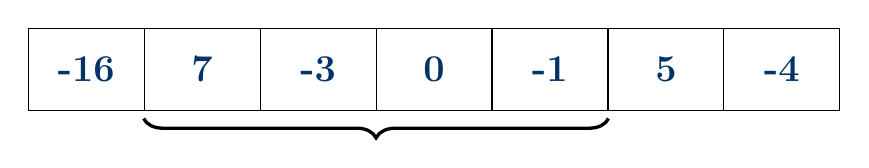
\begin{tikzpicture}[
		cell/.style={draw, minimum width=1.55cm, minimum height=1.1cm, align=center},
		num/.style={font=\bfseries\Large, text=HUSTBlue},
		brace/.style={decorate, decoration={brace, amplitude=7pt, mirror}, very thick},
		scale=0.95, transform shape
		]
		
		% ===== 7 ô số =====
		\foreach \v [count=\i from 1] in {-16,7,-3,0,-1,5,-4}{
			\node[cell] (A\i) at ({(\i-1)*1.55},0) {\textcolor{HUSTBlue}{\bfseries\Large \v}};
		}
		
		% ===== ngoặc lớn: từ 7 đến -1 (A2..A5) =====
		\draw[brace, black]
		($(A2.south west)+(0,-0.10)$) -- ($(A5.south east)+(0,-0.10)$);
		
	\end{tikzpicture}
	
	\vspace{0.55cm}
	
	{\large\bfseries\itshape
		Bài toán con: Tìm đoạn con cực đại của đoạn (7, -3, 0, -1)
	}
	
\end{frame}

\begin{frame}[t]{Ví dụ: Đoạn con có tổng lớn nhất}
	\small
	\setlength{\leftmargini}{-1.2em}
	
	\begin{itemize}
		\item \textbf{Chia:} Chia đôi dãy $n$ phần tử tại điểm đưa
		$\textit{mid}=\textit{round}\!\left(\dfrac{n+1}{2}\right)$
		\begin{itemize}
			\item Bài toán con 1: Giống bài toán cha, tìm dãy con cực đại của dãy $1,\ldots,\textit{mid}$
			\item Bài toán con 2: Giống bài toán cha, tìm dãy con cực đại của dãy $\textit{mid}+1,\ldots,n$
			\item Bài toán con 3: Tìm dãy con cực đại có chứa phần tử $\textit{mid}$ và không biết thành phần đầu tiên và
			cuối cùng
		\end{itemize}
	\end{itemize}
	
	\vspace{0.35cm}
	\centering
	
	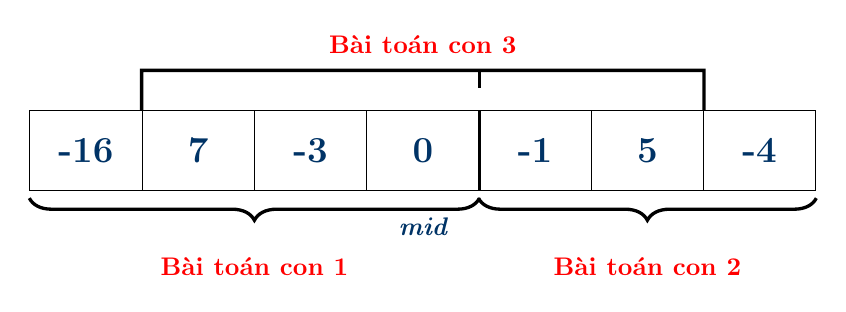
\begin{tikzpicture}[
		cell/.style={draw, minimum width=1.55cm, minimum height=1.1cm, align=center},
		num/.style={font=\bfseries\Large, text=HUSTBlue},
		bbrace/.style={decorate, decoration={brace, amplitude=8pt, mirror}, very thick},
		scale=0.92, transform shape
		]
		
		% ===== 7 ô số =====
		\foreach \v [count=\i from 1] in {-16,7,-3,0,-1,5,-4}{
			\node[cell] (A\i) at ({(\i-1)*1.55},0) {\textcolor{HUSTBlue}{\bfseries\Large \v}};
		}
		
		% ===== vạch chia tại mid (sau phần tử 0) =====
		\draw[thick] (A4.north east) -- (A4.south east);
		\node[HUSTBlue, font=\bfseries\itshape] at ($(A4.south)+(0,-0.5)$) {mid};
		% ===== ngoặc TRÊN: Bài toán con 3 (từ sau -16 đến trước -4) + "răng" ở mid =====
		\coordinate (L) at (A2.north west);     % biên giữa -16 và 7
		\coordinate (R) at (A6.north east);     % biên giữa 5 và -4
		\coordinate (M) at (A4.north east);     % đúng vị trí mid (sau 0)
		
		\coordinate (Ltop) at ($(L)+(0,0.55)$);
		\coordinate (Rtop) at ($(R)+(0,0.55)$);
		\coordinate (Mtop) at ($(M)+(0,0.55)$);
		
		\draw[very thick] (L) -- (Ltop) -- (Rtop) -- (R);
		\draw[very thick] (Mtop) -- ($(Mtop)+(0,-0.25)$);
		
		\node[red, font=\bfseries] at ($(Ltop)!0.5!(Rtop)+(0,0.35)$) {Bài toán con 3};
		
		% ===== ngoặc DƯỚI: Bài toán con 1 và 2 =====
		\draw[bbrace] ($(A1.south west)+(0,-0.10)$) -- ($(A4.south east)+(0,-0.10)$);
		\draw[bbrace] ($(A5.south west)+(0,-0.10)$) -- ($(A7.south east)+(0,-0.10)$);
		
		\node[red, font=\bfseries] at ($(A1.south west)!0.5!(A4.south east)+(0,-1.05)$) {Bài toán con 1};
		\node[red, font=\bfseries] at ($(A5.south west)!0.5!(A7.south east)+(0,-1.05)$) {Bài toán con 2};
		
	\end{tikzpicture}
	
\end{frame}

\begin{frame}[t]{Ví dụ: Đoạn con có tổng lớn nhất}
	\small
	\setlength{\leftmargini}{-1.2em}
	
	\begin{itemize}
		\item \textbf{Giải bài toán con:} Bài toán con 1 và 2 có thể giải bằng đệ quy.
		Bài toán con 3 giải được trực tiếp do có ràng buộc phải chứa phần tử \textit{mid}.
		Lời giải bài toán 3 là hợp của đoạn con cực đại kết thúc tại \textit{mid} và đoạn con cực đại bắt đầu từ
		\textit{mid + 1}. Để giải 2 bài toán nhỏ này, chúng ta chỉ cần duyệt từ \textit{mid} lùi về 1 và từ
		\textit{mid + 1} tiến về n, với độ phức tạp $O(n)$
	\end{itemize}
	
	\vspace{0.35cm}
	\centering
	
	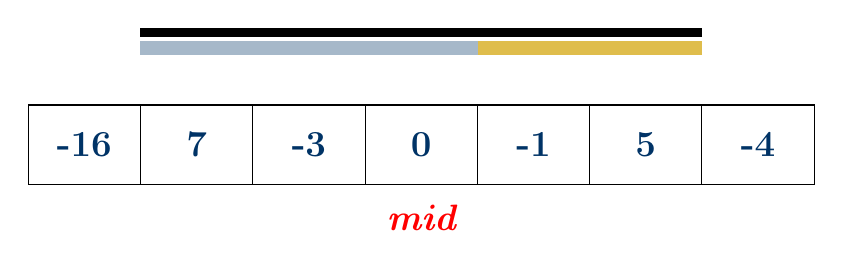
\begin{tikzpicture}[
		cell/.style={draw, minimum width=1.55cm, minimum height=1.1cm, align=center},
		num/.style={font=\bfseries\Large, text=HUSTBlue},
		scale=0.92, transform shape
		]
		
		% ===== 7 ô số =====
		\foreach \v [count=\i from 1] in {-16,7,-3,0,-1,5,-4}{
			\node[cell] (A\i) at ({(\i-1)*1.55},0) {\textcolor{HUSTBlue}{\bfseries\Large \v}};
		}
		
		% ===== chữ mid đỏ nghiêng dưới ô 0 =====
		\node[red, font=\bfseries\itshape\Large] at ($(A4.south)+(0,-0.45)$) {mid};
		
		% ===== thanh đen dài phía trên =====
		\draw[line width=3.2pt] ($(A2.north west)+(0,1.00)$) -- ($(A6.north east)+(0,1.00)$);
		
		% ===== 2 thanh màu (xanh + vàng) ngay dưới thanh đen =====
		\draw[line width=5.2pt, draw=HUSTBlue!35]
		($(A2.north west)+(0,0.78)$) -- ($(A4.north east)+(0,0.78)$);
		
		\draw[line width=5.2pt, draw=codegold!70]
		($(A4.north east)+(0,0.78)$) -- ($(A6.north east)+(0,0.78)$);
		
	\end{tikzpicture}
	
\end{frame}
\begin{frame}[t]{Ví dụ: Đoạn con có tổng lớn nhất}
	\small
	\setlength{\leftmargini}{-1.2em}
	
	\begin{itemize}
		\item \textbf{Xác định bài toán con:} Bài toán con của bài toán tìm đoạn con cực đại của dãy
		$(a_1,\ldots,a_n)$ là bài toán tìm đoạn con cực đại của đoạn con
		$a_i,a_{i+1},\ldots,a_{i+j},\, i \ge 1,\, i+j \le n$.
		
		\item \textbf{Chia:} Chia đôi dãy $n$ phần tử tại điểm đưa
		$\textit{mid}=\textit{round}\!\left(\dfrac{n+1}{2}\right)$
		\begin{itemize}
			\item Bài toán con 1: Giống bài toán cha, tìm dãy con cực đại của dãy $1,\ldots,\textit{mid}$
			\item Bài toán con 2: Giống bài toán cha, tìm dãy con cực đại của dãy $\textit{mid}+1,\ldots,n$
			\item Bài toán con 3: Tìm dãy con cực đại có chứa phần tử $\textit{mid}$ và không biết thành phần đầu tiên và cuối cùng
		\end{itemize}
		
		\item \textbf{Giải bài toán con:} Dùng đệ quy và duyệt mảng độ phức tạp $O(n)$
		
		\item \textbf{Tổng hợp:} Lời giải là lời giải tốt nhất trong 3 lời giải của 3 bài toán con
		
		\item \textbf{Độ phức tạp thuật toán:} $O(\log(n))$
	\end{itemize}
	
\end{frame}

\begin{frame}[t]{Ví dụ: Tính nhanh $a^n$}
	\small
	\setlength{\leftmargini}{-1.2em}
	\setlength{\itemsep}{0.75em}
	
	\begin{itemize}
		\item \textbf{Phát biểu:} Tính $a^n$ với $a$ và $n$ là các số nguyên dương
		
		\item \textbf{Phân tích:} Phương pháp trực tiếp, thực hiện $n$ phép nhân,
		có độ phức tạp tính toán $O(n)$. Chúng ta có thể làm tốt hơn với Thuật toán chia để trị?
		
		\item \textbf{Thiết kế thuật toán chia để trị:}
		\begin{itemize}
			\item \textbf{Bài toán con:} Tính $a^k, k < n$
			\vspace*{0.2cm}
			\item \textbf{Chia:} Ý tưởng chia đôi, 2 bài toán con giống hệt nhau, chỉ cần giải một bài toán con
			\begin{itemize}
				\item Nếu $n$ chẵn, ta có $a^n = \left(a^{\frac{n}{2}}\right)\times\left(a^{\frac{n}{2}}\right)$
				\item Nếu $n$ lẻ, ta có $a^n = a \times a^{n-1}$
			\end{itemize}
			\item \textbf{Xử lý:} Sử dụng đệ quy để giải
			\vspace*{0.2cm}
			\item \textbf{Tổng hợp:} Đơn giản, chỉ là một phép tính toán nhân
		\end{itemize}
		
		\item \textbf{Độ phức tạp thuật toán:} $O(\log(n))$
	\end{itemize}
	
\end{frame}


\begin{frame}[t,fragile]{Ví dụ: Tính nhanh $a^n$}
	\large
	\setlength{\leftmargini}{-1.2em}
	
	\begin{itemize}
		\item Code minh hoạ:
	\end{itemize}
	
	\vspace{0.55cm}
	\centering
	
	\begin{minipage}{0.78\textwidth}
		\begin{minted}[
			fontsize=\normalsize,
			frame=single,
			rulecolor=\color{codegold},
			framesep=6mm,
			numbers=none,
			autogobble=true,
			breaklines=false,
			escapeinside=||
			]{text}
			|\textcolor{HUSTBlue}{int}|  |\textcolor{HUSTBlue}{Pow}|(|\textcolor{blue}{int}| x, |\textcolor{HUSTBlue}{int}| n) {
				|\textcolor{HUSTBlue}{if}| (n == 0) |\textcolor{HUSTBlue}{return}| 1;
				|\textcolor{HUSTBlue}{if}| (n % 2 != 0) |\textcolor{HUSTBlue}{return}| x * |\textcolor{HUSTBlue}{pow}|(x, n - 1);
				|\textcolor{HUSTBlue}{int}| res = |\textcolor{HUSTBlue}{Pow}|(x, n/2);
				|\textcolor{HUSTBlue}{return}| res * res;
			}
		\end{minted}
	\end{minipage}
	
\end{frame}

\begin{frame}[t]{Bài tập luyện tập}
	\small
	\setlength{\leftmargini}{-1.2em}
	\setlength{\itemsep}{1.15em}
	
	\begin{itemize}
		\item \textbf{Ý tưởng:} Cài đặt thuật toán Sắp xếp trộn (Merge sort)
		
		\item \textbf{Đề bài:} Sắp xếp mảng gồm $n$ số nguyên sử dụng thuật toán chia để trị.
		Gợi ý, bài toán cha chia thành 2 bài toán con bằng nhau.
		
		\item \textbf{Hình thức:} Làm tại nhà và nộp lại trên hệ thống chấm code
	\end{itemize}
	
\end{frame}

























%Hết

{\HUSTUseBackground{theme_hust_oneside.pdf}
\begin{frame}
\ifdefstring{\insertaspectratio}{169}{
	\placecontent{0.355\paperwidth}{0.410\paperheight}{0.640\paperwidth}{
		\color{HUSTRed}\bfseries\fontsize{28pt}{36pt}\selectfont\centering
		THANK YOU!
	}
}{}
\ifdefstring{\insertaspectratio}{43}{
	\placecontent{0.355\paperwidth}{0.440\paperheight}{0.640\paperwidth}{
		\color{HUSTRed}\bfseries\fontsize{28pt}{36pt}\selectfont\centering
		THANK YOU!
	}
}{}
\end{frame}
}



\end{document}
